\chapter{Security for e-Government}
Security is a generic word used to describe the defense mechanism to be set in place by all users of ICT to ward off the attacks on their information assets-whether in storage or in transit - and to mitigate the impact in the event of an attack. Given the ingenuity of ICT users (abusers!), the attacks can happen in several forms and so the defense mechanisms have to be sufficiently strong and comprehensive.

%@Misc{noauthor_lists_nodate,
%	title = {lists - enumerate in multicols},
%	url = {https://tex.stackexchange.com/questions/67966/enumerate-in-multicols},
%	urldate = {2021-01-24},
%	journal = {TeX - LaTeX Stack Exchange},
%}
 \section{Challenges of e-government Security}
 As we know the e-Government provides services to citizen, business, employees and stores the data and information of almost all aspects of the government and the country, there is always danger of access by unauthorized people through hacking. There must be mechanism to provide security  so some of the challenges of e-Government security are as follows\cite{jayramChaulagain}:
 
 \subsection{Need for a Good User Experience}
  A good user experience is one of the factor conducive to the success of e-Government initiatives. The users can be internal users i.\ e.\ the employees of the agencies that operate and manage ICT systems at the backend, or the end users, i.\ e.\ citizens and businesses that access e-services. Both sets of these users want as few hassles as permissible while gaining access to system and services who want to do their work in few clicks. This requirement places serious limitations on the number and type of security controls that can be put into the system without loosing user interest.
  
  \subsection{Multiple Legacy Environments}
  Governments may have many legacy system each with own security sub-system. Creating a comprehensive security framework that can inter-operate between such diverse system can be a challenge. Similarly, multiple application system demand varying degrees of rigor in security implementations, depending on the varying threat perceptions. A blanket of security mechanism is not always the best.
  
  
 \subsection{Ever Expanding Domain of e-Government}
 With governments eager to deliver more and more services online to a larger client, the boundary that needs to be protected is ever-increasing and so also the nature and intensity  of attacks with which  the expanded domain is threatened. This adds a new dimension scalability of the security solutions designed in the preliminary stages.
 
 \subsection{Wide Range of Access Needs}
 The users within the government agencies are a peculiar lot. They need as much flexibility in their operations as in the paper-based system — if not more! Failure to realize this and provide for the same might act as a strong de-motivator. For instance, users would expect to access the backend system from anywhere and at anytime. They would like access to be provided at the workstation in the office and through the laptop while at home or on travel. They would like speech-recognition software to be deployed, so they can talk to the computer rather than type into it! These requirements bring in special vulnerabilities that need to be addressed by the security designers.
 
 
 
 \section{An Approach to Security for e-Government}
 A rational approach to security start with two questions -``security of what?'' and ``security against what?'' These are, incidentally, the two questions to be answered by any agency while undertaking the first steps in e-security - the self-assessment stage.
 
 \subsection{Security for What?}
 Security is all about safeguarding the ICT assets of an organization. The assets in the portfolio could be internal assets of the organization or external assets. While the internal assets are easy enough to visualize, the external assets that lie outside the `perimeter' of the organization include the assets of the clients, remote users and business partners who need to communicate and collaborate with the organization day in day out. The ICT assets themselves can be of a wide variety including the following:
 
 \subsubsection*{Data}
 Data in the form of data on the organization, its transactions, sensitive data relating to citizens and businesses such as the socio-economic data of citizens and business returns, data relating to properties of individuals and their titles and charges thereon, medical data of citizens, data of educational institutions and social security data. The data can be in individual databases, data marts or in data warehouse.
 
 
 \subsubsection*{Information}
 Information in the form of processed data, such as processed tax returns, driving licenses, medical claims, annual business returns, websites of agencies, directories of users, work-flow processes etc.
 
 \subsubsection*{Knowledge resources}
 E.\ g.\ patents, Acts, Rules and Regulations, research papers, reports, meta-data schema, standards and specification, most of which may contain valuable intellectual properties.
 
 
 \subsubsection*{Programs}
 Programs such as e-government applications that provide services to millions of citizens and thousands of businesses, operating systems, e-mail systems and web servers. Most of them contain thousands of person years of efforts behind them.
 
 \subsubsection*{Hardware}
 Hardware such as PCs, servers, routers, switches, data centers.
 
 \subsubsection*{Networks}
 E.\ g.\ LANs, WANs, and wireless networks.
 
 \subsection{Security against What?}
 The threat to security of ICT systems may come from many sources and in many forms. It is necessary to identify these threats, in the context of a particular e-government project or of the environment in general. What are the sources of threat to e-government?  The sources can be internal or external to the government agency.
 
 \subsection{Internal Sources of Threat}
 
 \subsubsection*{Government employees}
 Government employees working within e-government projects may misuse their access privileges to secure financial gains or disgruntled employees may try to sabotage the program to spite the government and/or to retain their vested interests.
 
 \subsubsection*{Employees of the private partners}
 Employees of the private partners of e-government operating the systems in a PPP arrangement may resort to such a misuse as above.
 
 \subsubsection*{Customers of the e-government programs}
 Customers of the e-government programs may attempt to access the databases for financial gains.
 
 
 \subsection{External Sources of Threat}
 
 \subsubsection*{Professional hackers}
 Professional hackers who have the requisite technical skills to break into e-government systems, are perhaps the biggest threat. They may not expect any financial or other gains but the sadistic pleasure of disrupting citizen services.
 
 \subsubsection*{Criminal organizations}
 Criminal organizations which are inimical\footnote{Not friendly} to the government.
 
 \subsubsection*{Terrorist organizations} 
 Terrorist organizations that want to destabilize economies predominantly dependent on digital systems.
 
 \subsubsection*{Intelligence and investigation agencies}
 Intelligence and investigation agencies that want to secure sensitive and classified information from government agencies.
 
 
 \subsection{What are the Types of Threats?}
 Threats to ICT assets may be of different types and varying intensities and impact values. As a  corollary\footnote{A practical consequence that follows naturally}, the attacks on security of systems can be in different forms including the following:
 
 \subsubsection*{Defacing of web sites}
 Defacing of websites and filling the home pages with objectionable material.
 
 \subsubsection*{Hacking into servers}
 Hacking into servers and stealing valuable data and information.
 
 \subsubsection*{Damage}
 Damage to critical databases and applications.
 
 \subsubsection*{Denial of Service Attack(DOS)}
 Denial of Service Attack (DOS), which involves flooding the government portals with millions of requests at business-critical hours to deny the service to genuine users.
 
 \subsubsection*{Virus attack}
 Virus attack directed against a particular government agency or broadcast without direction, which may have the effect of corrupting data or application programs and is usually associated with slowing down or even breakdown of networks.
 
 
 The damage to ICT assets need not always be a result of such malicious attacks as above. It can be occasioned by accident, incorrect usage of the systems. Can be a result of power fluctuations or outages, natural calamities such as floods, earthquakes, fire or vandalism.
 
 The UK Government, in its \textit{e-government Security Framework}, lists 18 types of attacks and threats to e-government assets.
 
 \begin{enumerate}
 	 \begin{multicols}{2}
 		\item Unknown outsider attacks
 		\item User fraud
 		\item Insider attack
 		\item Privileged insider attack
 		\item False identity 
 		\item Impersonation
 		\item Unauthorized disclosure
 		\item (Misuse of) revoked rights
 		\item Theft of access token
 		\item Duplication of access tokens 
 		\item Capture of access credentials
 		\item Denial of service attack
 		\item Misinformation and propaganda
 		\item Breach of anonymity
 		\item Breach of accountability
 		\item Failure to recover business information 
 		\item Loss or theft of monetary value
 		\item Challenges to system veracity\footnote{accuracy}
 	\end{multicols}
 \end{enumerate}

 \section{Security Management Model}
Security of e-government systems has to be managed systematically, comprehensively and continuously. Figure {\ref{fig:security-environment}} shows a model for understanding the various elements in such a security environment.
 
 %%%%%%%%%%%%%%%%%%%%%%%%%
 %						%
 %		Figure	  	 	%
 %						%
 %%%%%%%%%%%%%%%%%%%%%%%%%
 \begin{figure}[ht]
 	\centering
 	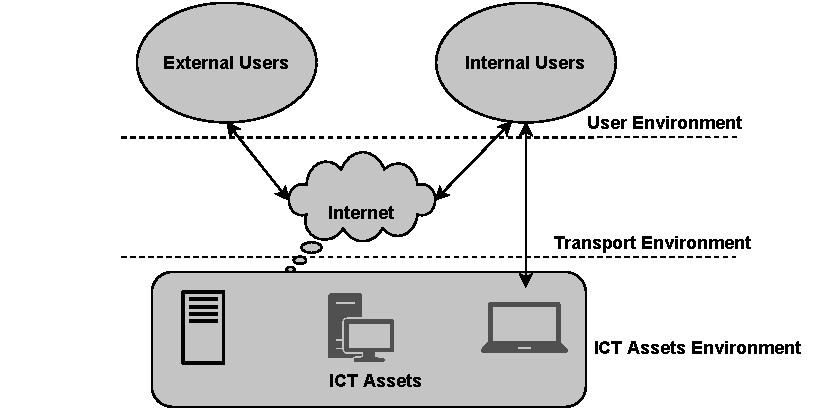
\includegraphics[width=\textwidth]{security-environment}
 	\caption{Security Environment.}\label{fig:security-environment}
 \end{figure}
 
The security environment consists of three distinguishable areas or environments,
each of which is subject to different types of threats and consequently needs different
security treatment:
\begin{itemize}
	\item The \textit{User Environment}
	\item The \textit{Transport Environment}
	\item The \textit{ICT Assets Environment}.
\end{itemize}
 
 Table {\ref{tab:security-model}} brings out the essence of the security model
 \begin{landscape}
 \begin{table}[ht]
 	\caption{Security Mode of e-Government.}\label{tab:security-model}
 	\begin{tabular}{p{5.5cm}p{5.5cm}p{5.5cm}}
 		\toprule
 		\textbf{Environment}                                                                    & \textbf{Management systems}                                                                              & \textbf{Management tools}                                                                                                                                                         \\ \midrule
 		{\bfseries User Environment\par}{$\bullet$ Internal users\par $\bullet$ External users} & {$\bullet$ Identity Management\par $\bullet$ Access Management\par $\bullet$ Interaction Management} & {$\bullet$ Passwords\par $\bullet$ Digital identity token\par $\bullet$ Access Control Lists (ACL)\par $\bullet$ PKI\par $\bullet$ Biometrics\par $\bullet$ e-government gateway} \\ \hline
 		
 		{\bfseries Transport Environment\par}{$\bullet$ Within LAN, WAN\par $\bullet$ Over the Internet} & {$\bullet$ Secure Communication System\par $\bullet$ Cryptographic Systems\par} & {$\bullet$ Government secure Intra-net\par $\bullet$ Virtual private networks\par $\bullet$ Government Secure Internet (GSI)\par $\bullet$ Encryption} \\ \hline
 		
 		 {\bfseries ICT Assets Environment\par}{$\bullet$ Tangible assets\par $\bullet$ Intangible assets} & {$\bullet$ Physical Security\par $\bullet$ Electronic Security\par} & {$\bullet$ Firewalls\par $\bullet$ Intrusion detection systems\par $\bullet$ Anti-virus systems\par $\bullet$ Disaster recovery site} \\ 
 		\bottomrule
 	\end{tabular}
 \end{table}
\end{landscape}
 
 From the security perspective, the e-government environment can be imagined to consist of three portions: 
 \begin{itemize}
 	\item the \textit{User environment}
 	\item the \textit{Transport environment} and
 	\item the \textit{ICT Assets environment}.
 \end{itemize} 
Users can be internal or external. Transport can be over private or public networks. ICT assets can be Tangible or Intangible.

\subsection{User Environment}
Security Management of user environment involves asking three basic questions of
individuals seeking to access the information system or to interact with it.
\begin{enumerate}
	\item \textit{Who are you?}
	\item \textit{What are you permitted to do with the system?}
	\item \textit{What are you accountable for in your interactions with the system?}
\end{enumerate}

 This is the objective of the three management systems shown in Table {\ref{tab:security-model}} -Identity Management Systems, Access Management Systems and Interaction Management Systems. 
 
 \subsubsection*{Identity Management Systems} 
 The objectives of an Identity Management System are:
 \begin{itemize}
 	\item To create unique \textit{digital identities} or credentials to all legal persons—citizens
 	and businesses—after establishing their existence and identifying them with
 	reference to name, date of birth, etc.
 	
 	\item To create and manage directories which link the digital identities with the real world identities and provide for their \textit{accessibility} to all other persons seeking to
 	communicate with them.
 	
 	\item  To create and manage ICT systems which ensure that the digital identities are \textit{secure}, i.\ e.\ they are not stolen, easily tampered with or ‘broken into'.
 	
	\item To \textit{revoke} the digital identity of a person when its confidentiality has been compromised or such identity is not otherwise required, by virtue of the death of such person or cessation\footnote{Put an end to an activity} in the role or office.
 \end{itemize}
 
 Examples of Identity Management Systems are:
\paragraph*{Username and password management system}

 A simple and `conventional' \textit{username and password} management system together with appropriate directory management services. The following
 guidelines are provided in this regard:
 
 \begin{enumerate}[label=(\alph*)]
 	\item Government agencies should \textit{clear-cut password policies} that prescribe things like the minimum password length, complexity of the password in terms of mandatory combination of alpha-numeric and special characters, life period of
 	a password that forces users to change the password, restriction on adopting the
 	same password time and again and procedures for revocation of password.
 	
 	\item It is advisable that the directory be maintained securely and centrally so that
 	it is available to all authorized users.
 	
 	\item Lightweight Directory Access Protocol (LDAP) compliance is preferable
 	when a very strong security is not required.
 	
 	\item Implement a fault-tolerant solution that provides $ 24 \times 7 $ availability of
 	directory services.
 	
 	\item Design and use a meta-data schema together with a taxonomy that prescribes
 	what information of the person is registered and in what uniform format and what
 	are the classes of users and their hierarchies. Omission in this regard could lead
 	to a serious confusion in the registration and retrieval processes as the
 	e-government systems scale up to a few thousand users.
 \end{enumerate}
 
 \paragraph*{Public Key Infrastructure}
 Public Key Infrastructure (PKI) is a more advanced system that not only
 contains an Identity Management System but also the features of the other two
 systems, viz.\ Access Management System and Interaction Management System.

 
 
 
 \subsubsection*{Access Management Systems}
 An Access Management System serves the following objectives:
 
 \begin{itemize}
 	\item It enables ICT systems to identify the user uniquely by matching the password, digital identity token or other device that carries the digital identity of the user with that registered in the system.
 	
 	\item It authorizes the user to perform only those tasks and transactions that are
 	predefined as per the privileges granted by the system administrator at the time
 	of registration or subsequently.
 	
 	\item It can maintain intelligence of users who try unauthorized access of tasks for
 	which they are not privileged. This would be available to the management for
 	review and remedy.
 \end{itemize}

\textit{Access Control Lists (ACLs)} and \textit{Advanced Access Control Lists} are industry
standards in this area.
 
 
 \subsubsection*{Interaction Management Systems}
 The objectives of interaction management are by far the most comprehensive and complex.
 They include assurance of the following principles of a comprehensive security, which are,
 in a way, the founding pillars of interaction management.
 
 \paragraph*{Authentication}
 Authentication or the assurance that the user is actually the person who s(he) claims to be.
 
 \paragraph*{Integrity} 
  Integrity or the assurance that the message or document sent or transaction effected\footnote{Settled securely and unconditionally} through an ICT system has not been tampered with, traveled from to destination safely and got stored therein securely.
  
  
  \paragraph*{Confidentiality}
  Confidentiality or the assurance that the content of the message or document sent
  or transaction effected has not been read by anyone else except the person to
  whom it has been sent.
  
  \paragraph*{ Non-repudiation}
  Non-repudiation or the assurance that the person who has transacted shall not
  repudiate the same at a later date.\\
  
  
  The above four axioms are fundamental to a secure digital environment and
  flourishing of e-government transactions. These are more significant for the e-government
  scenario because these four requisites are precisely needed for a whole gamut\footnote{A complete extent or range} of
  e-government transactions involving exchange of contracts, title deeds, issue of statutory
  certificates, financial transactions, filing of tax returns, approvals and sanctions accorded
  through a work-flow, etc. PKI is a mechanism that gives all the four assurances.
  
 \subsubsection*{Tools for User Management}
 \paragraph*{Username and Password system}
 Username and Password system is the conventional system of user management. It has
 several security issues. The user can compromise the password. The password can be
 hacked. The password can be transferred. It does not assure that the person keying in the
 password is the real-world person to whom it was assigned.
 
 \paragraph*{Digital identity token}
 A digital identity token is a popularly used device to overcome some
 shortcomings of a simple password. It is a photo ID card that also has the password
 embedded in it either magnetically or as a chip. It serves the dual purpose of controlling
 the physical access to the work premises and of controlling access to the ICT systems that
 the user is authorized to access. It is quite suitable for employees in corporate work
 environments. The digital identity token is not completely foolproof or transfer-proof
 because it depends on human intervention at the entry point through verification of the
 photo ID with the person's face.
 
 \paragraph*{Biometric device}
 A biometric device seeks to overcome the deficiencies of a token by using the
 physical features of a person, such as the fingerprint or iris to establish identity uniquely.
 These features are captured at the time of registration, converted into a code using certain
 algorithms and stored for comparison at the time of authentication. 
 
 \paragraph*{Public Key Infrastructure (PKI)}
 Public Key Infrastructure (PKI) is a technology that is based on the theory of cryptography or converting an intelligible text or digital content into a form that can be
 decrypted and read by the user or person to whom it is sent. PKI basically uses the
 concepts of \textit{Digital Signature Certificate}, \textit{Asymmetric Key Pair}, \textit{Public Key}, \textit{Private Key}, Digital Signature and Encryption. 
 
 \subparagraph*{Digital signature certificate}
 A digital signature certificate is a document issued by Certification Authority (CA), legally clothed with powers to do so, to a person, creating the digital
 identity of that person after satisfying that the person truly is who s(he)
 claims to be. The CA may employ a number of Registration Authorities (RAs) for
 conducting such verification and front ending the process of issuing digital
 signature certificates. The digital signature certificate also contains the \textit{public key}
 of the person, besides details like name, address, and date of
 validity of the certificate. The CA can revoke a digital signature certificate in case
 it is no longer required or the user violates the conditions of the certificate, such
 as compromising the \textit{private keys}.
 
 \subparagraph*{Asymmetric key pair}
 An asymmetric key pair is a set of two complimentary keys or codes, generated
 using an algorithm such that:
 \begin{enumerate}[label=(\alph*)]
 	\item  a text, document or message encrypted using one key can be decrypted only by the other key, and
 	\item it is not possible to derive one key from the other.
 \end{enumerate}

\subparagraph*{Public key}
A public key is that part of an asymmetric key pair that is displayed or published
for information and usage by public. It is a part of the PKI directory. The public key of a person is used by others to send an encrypted message
to that person. The public key of a person is also used by the recipient of a
message or document in verifying the digital signature of a person attached to a
message or document.


\subparagraph*{Private key}
A private key conversely is the second of the key pair that is to be retained and
stored confidentially by the holder of the digital certificate. The private key is
used by a person.
\begin{enumerate}[label=(\alph*)]
	\item to decrypt messages sent by others (using his or her public key), and
	\item to digitally sign a message or document.\\
\end{enumerate}
 
PKI, if implemented as part of a comprehensive security policy, can meet the
requirements of authentication, integrity, confidentiality and non-repudiation.

Setting up of PKI in a country involves the following steps:

\begin{steps}
	\item Enacting legislation required to give legal status to electronic transactions
	conducted in conjunction with PKI.
	
	\item Selection of agencies in the public and private sectors, which can be licensed to
	set up the required infrastructure and act as CAs, after conducting an audit of their
	capabilities and track record.
	
	\item Promoting the use of PKI for e-government, by taking up specific initiatives in the areas of taxation, customs clearances, land titles and such high-value, high-stake areas.
	
	\item Notifying the designated official or group within the agencies piloting the PKI
	within e-government as RAs.
	
	\item Perhaps, as may be required initially, to subsidize the cost of digital certificates
	to promote the concept, as otherwise, the cost of a certificate could be prohibitive
	at low volumes.
\end{steps}

Example of PKI: \textit{RSA Security}.

 \subsection{Transport Environment}
 Transport Environment includes all the space between the users internal and external and the ICT assets of the e-government system. The need for maintaining the authenticity, integrity and confidentiality of the information is as important here from the security point of view as in the other two environments. Transport Environment is also one over which the administrators of the e-government systems do not have a total control—physical or electronic.

 Transport Environment consists of the LANs, WANs, wireless and RF networks, satellite-based networks (VSAT) besides the Internet, which is a critical component the transport infrastructure. All the networks except the Internet can be secured through appropriate means, within the control of the administrators. There are \textit{three} popular ways of tackling the security issues arising out of the use of Internet:
 
 \begin{itemize}
 	\item Creating a Virtual Private Network (VPN) in the public domain
 	
 	\item Installing firewalls at each interface point between the Internet and the agency networks and
 	
 	\item Encrypting the data communicated over the Internet.
 \end{itemize}

\subsubsection*{Virtual Private Network (VPN)}
VPN is a secure network over an insecure network.
VPN technology involves creation of a secure, ‘private’ network—or a tunnel—in a public network to provide secure communications. VPNs provide confidentiality by
encrypting data sent over it. They provide integrity by using \textit{checksums} to ensure packets are not corrupt. VPNs verify the identity of the sender before establishing the connection with the agency intranet. They also have features that support access management and non-repudiation.

The benefits of VPN include cost savings, security that is better than in a purely
Internet-based communication channel and enable remote access of ICT resources without a dedicated connection.

VPN technology involves three components — a \textit{VPN client} software, a \textit{VPN gateway}
at the entry point of the agency or enterprise and a \textit{VPN management application} that
ensures the features of PKI are integrated. IPSec (Internet Protocol Security) is the protocol most commonly used in creating VPNs. At the client end, IPSec encrypts the data packets,
encapsulates them in an ESP (Encapsulating Security Payload), which is then enclosed in
an IP packet and transported. The process of ‘unpacketing’ and decrypting happens at the VPN gateway.

VPN is not an unmixed blessing. There are issues such as the following:

\begin{enumerate}
	\item The payload of security in encryption and decryption is heavy
	
	\item There are performance and QoS issues
	
	\item Prone to Denial of Service Attacks
	
	\item Scalability issues
	
	\item Management issues, especially those relating to client side
\end{enumerate}

\paragraph*{VPNs for e-Government}
\emph{e-government often involves establishing a secure connectivity between the HQs of various agencies and its remote field agencies, to support enterprise-wide applications. Establishing dedicated networks involves expense and time much beyond permissible limits. In such circumstances, VPN can be evaluated as a viable option.}

 \subsection{ICT Assets Environment}
 ICT assets are by far the most valuable and sensitive from the point of the enterprise. The hardware, the software, databases and knowledge is held centrally in the conventional EDP winds or in data centers. As shown in Table {\ref{tab:security-model}}, two broad categories of security treatments
 are required here—the \textit{physical security} and \textit{electronic security}.
 
 \subsubsection{Physical Security}
 \textit{Physical security} involves steps that guard against physical damage or loss, These steps include:
 
\begin{enumerate}
	\item Aggregation of the core ICT assets in highly guarded data centers, with restricted entry through biometric-controlled doors.
	
	\item Provision of dust-proof air-conditioned environment in the data centers,
	preferably built to industry standards, with raised floor, special cabling for power and communications, fire protection systems, alarms and closed-circuit TV
	monitoring of the premises, etc.
	
	\item Discouraging or prohibiting the use of USBs that are likely to infect the
	systems with viruses.
	
	\item Prohibiting the use of the assets of the system for personal e-mail and browsing.
	
	\item Providing fail-over and redundant systems to ensure $ 24 \times 7 $ availability and eliminating single points of failure.
	
	\item Rigorous and automated systems of backup and archival.
	
	\item Maintenance of audit logs and their review.
	
	\item Deployment of biometric-controlled access to workstations and applications.
	
	\item Provision of high quality UPS systems for guarding against power fluctuations and outages.
	
	\item Above all, mirroring of the core data and applications in a remote Disaster
	Management site.
\end{enumerate}
 
\subsubsection{Electronic Security}
 \textit{Electronic security} involves placing controls at all the digital entry and exit points to monitor the digital traffic that enters and goes out of the enterprise. The electronic security tools broadly fall under three categories:
 \begin{multicols}{2}
	\begin{itemize}
		\item Anti-virus systems
		\item Intruder detection systems
		\item Firewalls
	\end{itemize} 
 \end{multicols}

 \paragraph{Anti-virus systems}
 A computer virus is a malicious software program that is capable of attaching itself to executable files, data, hard disks or to removable disks and can execute itself repeatedly, replicate itself several times or propagate itself over networks without the knowledge or permission of the user. Such repeated execution, replication or propagation may have the dangerous effects, such as the following, in increasing degree of damage to the host system.
 
 \begin{itemize}
 	\item Occupying valuable disk space
 	\item Slowing down of the system due to excessive consumption of the memory
 	capacity
 	
 	\item Slowing down or clogging of networks
 	
 	\item Corruption of data residing on hard disks and other media
 	
 	\item Corruption and the consequent dysfunction of the application programs
 	
 	\item Infecting the other computer systems that the user’s system communicates with.
 \end{itemize}

Virus programs are written and propagated by their authors purely with malicious
intentions of causing inconvenience or damage to the targeted users or to the community
of computer users at large. The virus programs are also called \textit{malware}. Virus programs are
the instruments of cyber-terrorism and pose an unknown but serious threat to the security
of all computer systems. The computer community has to guard itself of the dangers posed
by the virus menace\footnote{threat} appropriately to protect the ICT assets and to provide
information and services in a reliable manner to the customers and to continue internal
operations without a break.

The other broad categories of malware programs are \textit{worms} and \textit{Trojan horses.}

\textit{Worms} are parasitic computer programs that replicate themselves without infecting other
computer files, either on the user’s computer or in the other systems to which the user is
connected over a network. 

A \textit{Trojan horse} is a computer program that pretends to be a
harmless program but actually executes certain actions that the user does not expect to do.
It is not a virus in the strict sense as it does not replicate itself.

\paragraph*{Types of viruses}
Computer viruses are as variant, stubborn and painful as their biological counterparts. It is
essential to know these broad categories to be wary of the possible consequences and
take preventive security measures.

\subparagraph*{Boot sector virus}
 \textit{Boot Sector Infector (BSI)} is a virus that gets access to and
resides in the boot sector or the area of the computer (usually on the hard disk) where the initial programs required to start a computer are stored. Whenever the
computer tries to read the boot program, the virus gets into the memory and executes itself
to gain control over all the computer operations. It can infect all the files and also
propagate over the network fast. It is quite a nasty species as it poses immense problems
to get rid of.

\subparagraph*{Macro virus}
A malicious program written in macro language (a language used to conduct repetitive tasks in a computer product, e.g. MS Word or Excel) that attaches
itself usually to Word documents and does its damage whenever the document is Opened
It also spreads to other document files. It can be highly annoying.

\subparagraph*{Encrypted virus}
A virus that propagates in an encrypted manner to escape
detection by the anti-virus software. The virus also carries its own decrypting algorithm. 
Each time it decrypts itself, it produces a different code that can cause the intended damage
to the system. By virtue of the unpredictable sequence of the decrypted code, the encrypted
virus escapes detection. Variants of the encrypted virus are the:
\begin{itemize}
	\item \textit{Polymorphic virus }(which
	creates varied versions of itself, but containing its original potential to damage),
	\item \textit{Mutating virus} (which mutates or changes as it progresses through its course in the host system),
	\item \textit{Self-encrypting virus} (which encrypts its signature code differently each time it infects),
	\item \textit{Self-garbling virus} (which garbles its code when it is in transmission, but ‘degarbles’ itself when the host program has infected runs) and
	\item \textit{Stealth virus} (which intercepts the disk
	access requests made by the anti-virus programs and feeds them a clean image of the
	infected file to indicate the file size as it was before infection).
\end{itemize}
All these categories of viruses are intended to deceive the anti-virus software, conceal themselves in different ways, escape detection and proliferate\footnote{Grow rapidly}.

\subparagraph*{Anti-antivirus viruses}
These are virus programs that infect and disable specific
anti-virus programs installed on a system and thereby continue their damage.

 \subparagraph*{Antivirus virus}
 These are viruses that specifically look for and remove other viruses.
 
 
\paragraph*{Relevance of anti-virus software to e-government}
Securing e-government systems from viruses is extremely important for the following
reasons:
 \begin{itemize}
 	\item \textit{Availability} of e-services on a $ 24 \times 7 $ basis is a requisite. e-government systems 
 	cannot be shut down for disinfection as it would adversely affect the reliability.
 	\item \textit{Trust and confidence} of the citizens would be shattered if the valuable
 	transactions recorded by them in e-government systems get corrupted or obliterated\footnote{Reduced to nothingness} due to virus attack.
 	\item Several \textit{sensitive} functions would be seriously affected in the event of a virus
 	attack.
 	\item e-Government systems have special \textit{vulnerability} from the point of view attacks by authors of viruses.
 \end{itemize}

\paragraph*{Anti-virus techniques}

\subparagraph*{Prevention}
 Agencies and enterprises should have rigid and clear virus prevention policy as part of their overall security policy. It should lay down severe restrictions on the usage of USBs, downloading pirated games or games and programs from untrusted sites and other potentially virus-carrier programs, send timely alerts to all users against opening e-mail suspected to carry virus, and do regular scanning of all systems and so on.


 \subparagraph*{Protection} 
Defense in depth and an integrated
solution are recommended practices in virus protection. The defense in depth method involves appropriate steps and solutions at three levels, namely, the \textit{user level}, the \textit{backend systems level} and \textit{perimeter level}. 

\subsubsection{Intrusion Detection Systems}
Intrusion Detection Systems (IDS) are automated monitoring systems that watch for
abnormal, unauthorized or malicious activities. The role of IDS is to watch the traffic
patterns, analyze traffic content, review the firewall log files and monitor user account
activity. IDS can warn system administrators when an attack or intrusion is taking place.

Depending on the sophistication of the IDS, it can be configured to repel attacks on the fly
or track down the origin of the attack. It is not strictly required to protect the network from
Internet-based attacks, but it does provide a more extensive and automated monitoring
system. Repeated unsuccessful attempts to access the systems, accessing the systems
apparently by registered users but at unexpected hours or from different locations,
unprecedented high volume of traffic coming from a particular source, etc.\ are enough
reasons for the IDS to suspect a security breach and to alert the administrators.

\subsubsection{Firewalls}
Firewall is a computer system or a group of systems hardware and software that an access control policy between two separate networks, such as between two LANs or two WANs or a LAN and a WAN or most usually between a LAN/WAN and the Internet. The key feature about a firewall is that is only a mechanism to enforce the access control policy of the agency. The prerequisite for the successful deployment of a firewall, therefore, is the design and promulgation of an enterprise security policy. Firewall serves the basic purpose of making it nearly impossible for unauthorized users to access the ICT assets (situated `behind' the firewall) while permitting the authorized users to access the same effortlessly.

Firewalls typically adopt the following techniques for the ‘inspection’ required for
implementing the security regime. An understanding of these techniques enables
e-government managers to better manage the security policy.

\paragraph*{Packet filtering}
The firewall filters the IP packets with reference to the do’s and
don’ts or security rules prescribed by the organization. It validates the intelligence
it gathers from each packet against such rules.

\paragraph*{Network Address Translation (NAT)}
Firewalls also translate or replace the
internal or private IP numbers assigned to systems within the network with its
own public IP address so that the individual systems within the LAN of the
enterprise are not visible to the outside world and are more secure to that extent.

\paragraph*{Application proxy or proxy server}
A firewall can also act as a proxy of the
systems within the network, when such systems want to interact with the outside
world for such services as e-mail, Internet access, file transfer, etc. A proxy server
acts as a buffer between the internal workstations and the Internet.

\paragraph*{Logging and monitoring}
Firewalls have features that keep a record of the
events that happen within its purview. All exceptional or abnormal events are so
logged, for review by the security administrators. In the event of a high risk anticipated at the firewall, it is programmed to send appropriate alerts to the
security administrators for prompt remedial action. For instance, when the
firewall suspects a ‘sniffing’ or pre-attack surveillance by an outsider, it sends such an alert.

\paragraph*{Content filtering}
Firewalls use the technique of content filtering to block
objectionable sites being accessed by the users or messages containing predefined
objectionable or obscene words being sent out of the system or received into it.

\paragraph{Types of Firewalls}
Firewalls are basically of two types: \textit{hardware firewalls} and \textit{software firewalls}.

\subparagraph{Hardware Firewalls}
These are security appliances that contain the hardware and
software bundled into one. The firewall software is preloaded into the appropriately sized
hardware and configured for optimum performance with the result that the setup is quite
quick. Hardware firewalls are the preferred option when an organization wants to put in
place a security system quickly following a serious attack. Hardware firewalls tend to be
more expensive and less flexible as compared to software firewalls.

\subparagraph{Software firewalls}
These are software packages that need to be installed on the
existing hardware of the enterprise or hardware procured separately for the purpose. Due
to the availability of a wide range of software firewall products in the market, this would
be a preferred solution when the security needs of the agency are specific. Software
firewalls are less expensive, but require more time for installation and user training. There
are also personal firewalls for free download, which are suitable for standalone PCs.



\section{e-Government Security Architecture}
 Security Architecture is a high level document that directs and guides the security  efforts of individual e-Government initiatives and projects setting out the security objectives and goals, prescribing the standards to be achieved and indicating the procedures and processes that need to be followed by all the players participating in e-government, users, citizens, businesses, e-government partners, operators and service providers.
 
 The goals of the security architecture are to:
 \begin{itemize}
 	\item Create the necessary levels of confidence and trust among the stakeholders-citizens, businesses and government users.
 	\item Enforce global standards of security practice and implementation in e-Government.
 	\item Create and enforce digital identities including registration and enrollment as a means of accessing electronic government services.
 	\item Strengthen the four pillars of security i.\ e.\ \textit{authentication}, \textit{integrity}, \textit{confidentiality} and \textit{non-repudiation}.
 	\item Enhance the security awareness among the users through dissemination of a set of security guidelines.
 	\item Promote the development of operational schemes called security policies by individual government agencies.
 \end{itemize} 

 Security architecture seeks to achieve the above objectives by addressing the regulatory, technological and managerial issues arising out of the security needs and requirements of
 \begin{multicols}{2}
	\begin{itemize}
		\item user environment
		\item transport environment
		\item ICT assets environment.
	\end{itemize} 
 \end{multicols}


The security architecture, usually accompanied by a set of security guidelines, contains the following:
\begin{itemize}
	\item A description of the security environment consisting of the three portions mentioned above and what the e-government assets are the need to be secured and what the perceived security threats are.
	
	\item A description of the security requirements in functional and technical terms.
\end{itemize}

Any national or state government, intending to take up an e-government initiative seriously, should design an appropriate Security Architecture and Framework as a first step. This sets up the security vision in clear terms.

The formulation of a Security Architecture and Framework has to be quickly followed by three more initiatives:

\begin{itemize}
	\item Providing a \textit{statutory basis} for the e-government security architecture and mandating the security requirements on agencies that are partners in e-Government.
	\item Defining \textit{security standards} to be followed.
	\item Encouraging individual agencies in the public and private sectors to design appropriate \textit{security policies} that give a concrete shape to the manner of implementing the architecture in specific relation to the particular agency or enterprise.
\end{itemize}
 
 \section{Security Standards}
 The standards for information security was set up by the \textit{British Standard BS 7799}, which on account of its immense popularity was adopted by the ISO as \textit{IS0 17799}. There is also a sequel \textit{BS 7799-2} that prescribes the specification for Information Security Management.
 
 The versions of these security standards are \textit{ISO/IEC 17799}, which is the Code of practice for Information Security Management, and \textit{BS7799-2:2002} which gives the Specification for Information Security Management.
 
\textit{ISO/IEC 1799} is a standard that sets out the requirements for an Information Security Management. It helps identify, manage and minimize the range of threats to which information is regularly subjected. It defines 127 security controls structured under 10 major headings to enable the IS managers to identify the particular safeguards that are appropriate to their particular business or specific area of responsibility. 

\textit{BS7799-2:2002} tells us how to apply \textit{ISO/IEC} 17799 and how to build, operate, maintain and improve an ISMS.

The 10 major security areas identified by \textit{ISO/IEC 1799} and the ISMS methodology of implementing the security are mentioned briefly below, as they are central to an e-Government security policy.

\subsection[ISO/IEC 17799]{Ten Controls Prescribed By ISO/IEC 17799}
\begin{enumerate}
	\item \textit{Security policy}: Provides management direction and support for information security.
	
	\item \textit{Personal security}: Reduces the risks of human error, theft, fraud or misuse of facilities.
	
	\item \textit{Access control}: Secures management of access to information.
	
	\item \textit{Compliance}: Avoids breaches of any criminal and civil law, statutory, regulatory or contractual obligations, and any security requirement.
	
	\item \textit{Systems development and maintenance}: Ensures that security is built into information systems at the design and development stage.
	
	\item \textit{Communications and operations management}: Ensures the correct and secure operation of information communication and processing facilities.
	
	\item \textit{Organization of assets and resources}: Helps manage information security within the organization.
	
	\item \textit{Asset classification and control}: Helps identify assets and protect them appropriately.
	
	\item \textit{Physical and environmental security}: Prevents unauthorized access, damage and interference to business premises and information.
	
	\item \textit{Business continuity management}: Avoids interruptions to business activities and protects critical business processes from the effects of major failures or disasters.
\end{enumerate}

We can see that
\begin{itemize}
	\item the first five controls relate to the user environment
	\item the sixth one to transport environment and
	\item the remaining four to the ICT assets environment.
\end{itemize}
 
\subsection[ISMS]{Information Security Management System (ISMS)}
The information Security Management System (ISMS), also called Information Security Policy, is a document prepared by a government or an agency and addresses the following questions:

\begin{itemize}
 \item Why is information security important in the context of the e-government program or initiative?
 
 \item What are the threats perceived to be important? What are the possible attacks? What is the level of risk that the agency can accept or tolerate?
 
 \item What are the environments that we want to protect? In other words, who are the users, what are the communication channels, and what are the ICT assets that we want to protect? List, identify and classify them.
 
 \item What are the roles and privileges that we want to give to the users of various categories? Who is allowed to do what? What is the policy of the enterprise for e-mail, chat, web access, system administration, development and maintenance?
 
 \item How do we want to treat or manage the risks identified with the controls selected? In other words, what tools do we intend using for treatment of risks?
 
 \item What are the organizational arrangement that ensure management of the security policy and its continuous review and audit?
\end{itemize}

The ISMS of Information Security Policy is a working document that guides, instructs and canalizes the actions and efforts of all users of the ICT systems. Figure {\ref{fig:pdca-model}}, adopted from the Standard, defines a PDCA or Plan-Do-Check-Act cycle for management of the security.

%%%%%%%%%%%%%%%%%%%%%%%%%
%						%
%		Figure	  	 	%
%						%
%%%%%%%%%%%%%%%%%%%%%%%%%
\begin{figure}[hpb]
	\centering
	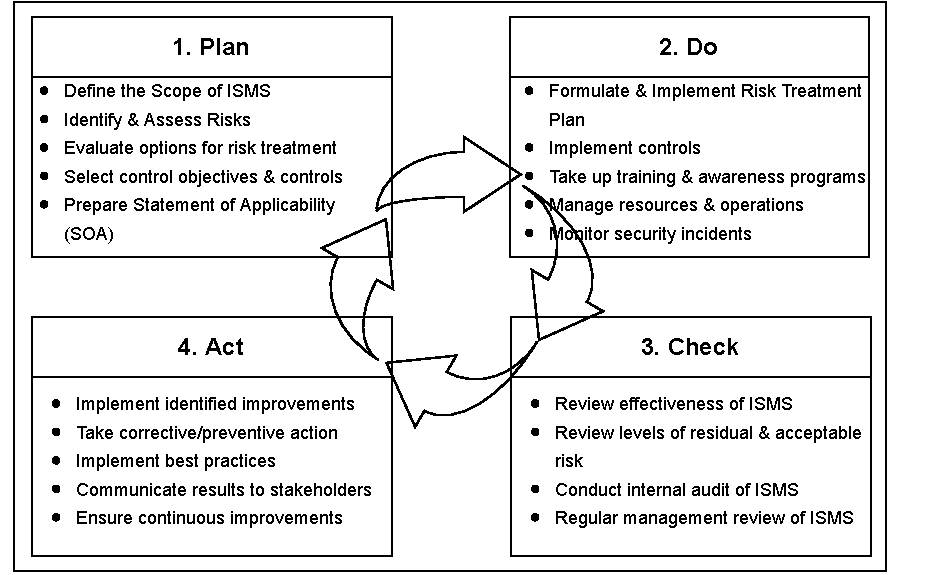
\includegraphics[width=0.8\textwidth]{pdca-model}
	\caption{The PDCA Model of Security Management.}\label{fig:pdca-model}
\end{figure}

 
Information Security is quite critical to the success of e-Government. We need a comprehensive security approach that spans across the user, transport and ICT assets environments. Publication of an e-government security architecture and preparation of an Information Security Management System, in conformity with the international standards are the most desirable practices.




 